\documentclass[twocolumn]{article}
\usepackage[english]{babel}
\usepackage[utf8]{inputenc}
\usepackage{amsmath,amssymb,physics,blindtext,graphicx}
\usepackage[a4paper,total={7.5in,10in}]{geometry}

\begin{document}
\begin{large}
\section*{Alpha decay and quantum tunnelling}
\subsection*{Description of the model}
Alpha decay is one of the most common nuclear decay process in which a (heavy) nucleus emits an alpha particle which is composed of two protons and two neutrons. In one of the simplest models, the alpha particle is in a potential well inside the rest of nucleus due to the strong interaction. When the distance between the alpha particle and the rest of the nucleus becomes large enough, the Coulomb interaction becomes dominant and the charged particles repel each other. However, the alpha particle has a non-zero probability of tunnelling through the Coulomb barrier and escape, leaving a daughter nucleus with two less protons and two less neutrons. The probability of tunnelling through the Coulomb barrier can be estimated, with some simplifying assumptions, by solving the one dimensional stationary Schrödinger equation:
\begin{equation}
    \label{26mar1229}
    \frac{\hbar}{2m_\alpha}u''(r) + (V(r)-E)u(r) = 0
\end{equation}
where $r$ is the distance between the particles, $m_\alpha=4$ u is the mass of an alpha paricle, $E$ is the energy which is measured experimentally and $V$ is the potential function. In this report, a description will be given on how this equation was solved numerically for the following alpha decays: 
\begin{itemize}
    \item[] $^{232}$Th $\to$ $^{228}$Ra, $E = 4.0$ MeV, $T_{1/2} = 4\cdot 10^{17}$ s,
    \item[] $^{220}$Ra $\to$ $^{216}$Po, $E = 6.4$ MeV, $T_{1/2} = 56$ s,
    \item[] $^{212}$Po $\to$ $^{208}$Pb, $E = 8.7$ MeV, $T_{1/2} = 3\cdot 10^{-7}$ s.
\end{itemize}
Here, $T_{1/2}$ are the experimentally verified half lives of the nuclei. The solution was used to find the probability of tunnelling through the barrier $T$, also called the transmission constant, which in turn gave the half lives according to this simplified model. These are then compared to the values above. The relationship between the transmission constant and the half life is given by:
\begin{equation}
    \label{28mar2156}
    T_{1/2} = \frac{\ln 2}{Tf}
\end{equation}
where $f$ is the frequency of the alpha paricle "hitting the wall" of the Coulomb barrier and can be estimated by with the velocity $v$ of the alpha particle: $f = v/2R = \sqrt{2E/m_\alpha}/2R$. 

\subsection*{Numerical methods for the problem}
It proved convenient to write the differential equation \eqref{26mar1229} in the dimensionless form: 
\begin{equation}
    \label{26mar1412}
    \begin{split}
        &u''(\xi) + \frac{2m_\alpha D^2U}{\hbar^2}(V'(\xi)-E')u(\xi) \\ 
        &\hspace{-0.6cm}=  u''(\xi) + \alpha(V'(\xi)-E')u(\xi) = 0 
    \end{split}
\end{equation}
where $\xi=r/D$, $V'=V/U$ and $E'=E/U$. The constants $D$ and $U$ are in the units of length and energy, respectively, which makes the constant $\alpha$ dimensionless. Suitable choices for $D$ and $U$ for this particular problem were $D=1$ fm and $U=1$ MeV. 
The potential is given by
\begin{equation}
    V(r) = 
    \begin{cases}
        -V_0 + V_C(R), \quad r < R \\
        V_C(r), \qquad\qquad\,\, r\geq R
    \end{cases}
\end{equation}
where $V_C$ is a discretized Coulomb potential between the alpha particle and the daughter nucleus: 
\begin{equation}
    V_C(r) = \frac{2(Z-2)e^2}{4\pi\epsilon_0r_j},\quad r_j\leq r < r_{j+1},
\end{equation}
and $r_j = R+(j-1)\Delta r$ with $j=1,2,\dots$ (see figure \ref{28mar2237}). The interval size $\Delta r$ is fixed and equal to the length of one barrier segment. The number of such barrier segments is designated by $N$. The value of $V_0$ is estimated\footnote{Buck, B., Merchant, A. C., \& Perez, S. M. (1990). New look at $\alpha$ decay of heavy nuclei. Physical review letters, 65(24), 2975} to be $V_0 = 134$ MeV and the radius $R$ of the well is given by the relationship:
\begin{equation}
    R = R_0\left(4^{1/3} + (A-4)^{1/3}\right)
\end{equation}
where $A$ is the mass number of the parent nucleus and $R_0 \approx 1.3$ fm. 

\begin{figure}[t]
    \centering
    \includegraphics[scale=0.5]{setup.png}
    \caption{The discretized potential of the problem. The number of barrier segments for this potential is $N=3$ and the number of intervals after the barrier is $M=1$.}
    \label{28mar2237}
\end{figure}
Since the potential is constant on the interval $(\xi_j,\xi_{j+1}) = (r_j/D,r_{j+1}/D)$, the solution on this interval is of the form:
\begin{equation*}
    u(\xi) = 
    \begin{cases}
        A_je^{i\omega_j\xi}+B_je^{-i\omega_j\xi},\quad E'>V'(\xi_j) \\ 
        A_je^{\omega_j\xi}+B_je^{-\omega_j\xi},\quad\,\, E'<V'(\xi_j) \\ 
    \end{cases}
\end{equation*}
where $\omega_j = \sqrt{\alpha|V'(\xi_j)-E'|}$. When $j=N+1$, the potential has dropped below the total energy (the potential was slightly shifted so that $V(\xi_j)\neq E$). The number of potential segments which lie below the total energy is designated by $M$. In the last region, $\xi\geq\xi_{N+M}$, it is assumed that the wave function is an outgoing wave:
\begin{equation*}
    u(\xi) = Fe^{i\omega_{N+M}\xi},\quad \xi\geq \xi_{N+M}.
\end{equation*}
The unknowns $A_j$, $B_j$ and $F$ are in total $2(N+M)+1$ and can be found by imposing continuity of $u$ and its derivative at the interfaces of the potential, $\xi_j$. That gives $2(N+M)$ equations but since \eqref{26mar1229} is a linear differential equation, we can set $A_0 = 1$ for instance. The linear system was solved for different values of $Z$ and $A$ which corresponded to the three different nuclei mentioned above. The transmission constant $T$ was calculated with 
\begin{equation}
    T = \frac{|F|^2}{|A|^2}\cdot\frac{\omega_{N+M}}{\omega_0}
\end{equation}
and the half life with equation \eqref{28mar2156}. This was done for a couple of  different values of $R_0$ around $1.3$ fm. Also, the dependece of $T$ on the number of segments after the barrier, $M$, was investigated. 
\subsection*{Results}
The half lives for the three nuclei as a function of $N$ can be seen in figure \ref{28mar2242}. For small $N$, the half lives are very sensitive to variations in $N$ but seem to converge for larger $N$. They also vary by orders of magnitude with small variations in $R_0$. As $R_0$ gets smaller, the Coulomb barrier gets higher and thus one would expect the transmission coefficient to decrease, and hence the half life to increase, which is what is observed. By varying $R_0$ it was possible to make the half lives converge to their experimental values. For a given $N$, it was found that the half life depended on the number of intervals after the barrier, $M$. For small $N$ it was found that increasing $M$, the half lives converged to a fixed value. Of course, for smaller $N$, the intervals are longer and the longer range effects of the Coulomb potential can be more easily taken into account. For larger $N$, however, the intervals are smaller and it's more 

\begin{figure}
    \centering
    \includegraphics[scale=0.4]{232Th_Thalf.png}
    \includegraphics[scale=0.4]{220Ra_Thalf.png}
    \includegraphics[scale=0.4]{212Po_Thalf.png}
    \caption{The half lives of $^{232}$Th (top), $^{220}$Ra (middle) and $^{212}$Po (bottom) calculated using the quantum tunnel model of alpha decay. The experimental values of the half lives are included.}
    \label{28mar2242}
\end{figure}
\newpage computationally expensive to take longer range effects into account. The accuracy of approximating the Coulomb potential is on the other hand increased. Perhaps it would be a good idea to use adaptive sized intervals which increase with larger distances. 

\begin{figure}[t]
    \centering
    \includegraphics[scale=0.4]{212Po_convergence.png}
    \caption{The half life of $^{212}$Po for few barrier segments $N$. As more intervals are taken into account, the half lives seem to converge.}
\end{figure}


\end{large}
\end{document}
